% Plain-English reading of Diagonal Archive Geometry.
% pdflatex plain_english.tex (twice for TOC).
\documentclass[11pt,a4paper]{article}

% ── Page & type ──────────────────────────────────────────────
\usepackage[margin=1.15in,marginparwidth=0pt]{geometry}
\usepackage[T1]{fontenc}
\usepackage{mathpazo}
\usepackage[scaled=0.92]{helvet}
\usepackage{microtype}
\usepackage{setspace}
\setstretch{1.15}
\setlength{\parskip}{0.4em}
\setlength{\parindent}{0pt}
\raggedbottom

% ── Colour (restrained ink) ──────────────────────────────────
\usepackage{xcolor}
\definecolor{ink}{HTML}{1A1A1A}
\definecolor{muted}{HTML}{5A5A5A}
\definecolor{rule}{HTML}{C8C4BC}
\definecolor{accent}{HTML}{2C3E50}
\definecolor{soft}{HTML}{F4F1EC}
\definecolor{nodefill}{HTML}{F7F5F1}
\definecolor{nodeedge}{HTML}{3D4F5F}
\color{ink}

% ── Math & lists ─────────────────────────────────────────────
\usepackage{amsmath,amssymb}
\usepackage{enumitem}
\setlist[itemize]{leftmargin=1.4em,itemsep=0.15em,topsep=0.3em}
\setlist[enumerate]{leftmargin=1.6em,itemsep=0.12em,topsep=0.3em}

% ── Tables, graphics, layout ─────────────────────────────────
\usepackage{booktabs}
\usepackage{tabularx}
\usepackage{graphicx}
\usepackage{tikz}
\usetikzlibrary{arrows.meta, positioning, calc}
\usepackage[skins,breakable]{tcolorbox}
\usepackage{titlesec}
\usepackage{fancyhdr}
\usepackage{caption}
\usepackage{needspace}
\usepackage{hyperref}
\hypersetup{
  colorlinks=true,
  linkcolor=accent,
  urlcolor=accent,
  pdfauthor={DAG},
  pdftitle={Diagonal Archive Geometry --- A Plain English Reading}
}
\captionsetup{font=small, labelfont={sf,bf}, textfont={it}, skip=0.4em}

% Keep diagrams with their prose (no floating away)
\newcommand{\figblock}[2]{%
  \begin{center}
  #1\\[0.35em]
  {\small\textit{#2}}
  \end{center}%
}

% ── Section styling ──────────────────────────────────────────
\titleformat{\section}
  {\Large\bfseries\color{accent}\sffamily}
  {\thesection.}{0.6em}{}
  [\vspace{-0.35em}{\color{rule}\titlerule[0.6pt]}]
\titleformat{\subsection}
  {\normalsize\bfseries\color{accent}\sffamily}
  {\thesubsection}{0.5em}{}
\titlespacing*{\section}{0pt}{1.25em}{0.55em}
\titlespacing*{\subsection}{0pt}{0.9em}{0.35em}

% ── Header / footer ──────────────────────────────────────────
\pagestyle{fancy}
\fancyhf{}
\renewcommand{\headrulewidth}{0pt}
\fancyfoot[C]{\color{muted}\small\thepage}
\fancyhead[L]{\color{muted}\scriptsize Diagonal Archive Geometry}
\fancyhead[R]{\color{muted}\scriptsize A plain-English reading}
\renewcommand{\headrulewidth}{0.4pt}
\renewcommand{\headrule}{\hbox to\headwidth{\color{rule}\leaders\hrule height \headrulewidth\hfill}}

% ── Custom environments ──────────────────────────────────────
\newtcolorbox{epigraphbox}{
  colback=soft,
  colframe=rule,
  boxrule=0pt,
  borderline west={2.5pt}{0pt}{accent},
  arc=0pt,
  outer arc=0pt,
  left=14pt, right=12pt, top=9pt, bottom=9pt,
  fontupper=\large\itshape\color{ink}
}

\newtcolorbox{claimbox}{
  colback=white,
  colframe=accent,
  boxrule=0.6pt,
  arc=1pt,
  left=12pt, right=12pt, top=7pt, bottom=7pt,
  fontupper=\large\color{accent},
  before skip=0.55em,
  after skip=0.55em
}

\newtcolorbox{principle}[1]{
  enhanced,
  breakable,
  colback=white,
  colframe=rule,
  boxrule=0.5pt,
  arc=2pt,
  left=10pt, right=10pt, top=7pt, bottom=7pt,
  before skip=0.65em,
  after skip=0.55em,
  title={\sffamily\bfseries #1},
  fonttitle=\normalsize,
  coltitle=accent,
  colbacktitle=soft,
  attach boxed title to top left={yshift=-2mm, xshift=8pt},
  boxed title style={
    colframe=rule, boxrule=0.4pt, arc=1pt,
    left=6pt, right=6pt, top=2pt, bottom=2pt
  }
}

\newcommand{\term}[1]{\textbf{#1}}
\newcommand{\Neg}{\ensuremath{\neg}}
\newcommand{\hrthin}{\par\vspace{0.35em}{\color{rule}\hrule height 0.4pt}\vspace{0.55em}}

\begin{document}

% ════════════════════════════════════════════════════════════
% Title
% ════════════════════════════════════════════════════════════
\begin{center}
  {\color{rule}\rule{0.55\textwidth}{0.6pt}}\\[0.9em]
  {\sffamily\LARGE\bfseries\color{accent} Diagonal Archive Geometry}\\[0.45em]
  {\large\color{muted} A plain-English reading}\\[0.7em]
  {\color{rule}\rule{0.35\textwidth}{0.4pt}}
\end{center}

\vspace{0.35em}

\begin{epigraphbox}
In one sentence.\quad
Reality is the unique minimal self-distinguishing process;
self-reference forces endless expansion;
preserved distinctions become archives;
archives generate the appearance of time;
and the true subject is the act of distinction itself
rather than anything distinguished.
\end{epigraphbox}

\vspace{0.25em}
\begin{center}
  {\color{muted}\small\textit{What the theory claims, before the formal machinery.}}
\end{center}

\vspace{0.4em}
\noindent{\sffamily\bfseries\color{accent} Contents.}
{\color{muted}\small\quad
1~Act \textperiodcentered\
2~Symmetry \textperiodcentered\
3~Survivor \textperiodcentered\
4~Dynamics \textperiodcentered\
5~Blind spot \textperiodcentered\
6~Growth \textperiodcentered\
7~Archives \textperiodcentered\
8~Time \textperiodcentered\
9~Subject \textperiodcentered\
10~Physics
}

\vspace{0.3em}
{\color{rule}\hrule height 0.4pt}
\vspace{0.5em}

% ════════════════════════════════════════════════════════════
\section{The primitive is an act}
% ════════════════════════════════════════════════════════════

\begin{principle}{Principle 1}
Reality originates from an \term{act}, not from a static entity.
\end{principle}

The primitive element is not matter, energy, space, information, or consciousness.

It is the simplest possible act: the \term{act of distinction}.

\figblock{%
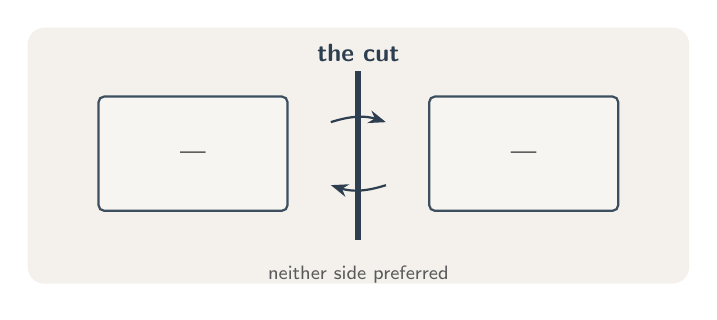
\begin{tikzpicture}[
  font=\small\sffamily,
  every node/.style={align=center}
]
  \fill[soft, rounded corners=6pt] (-4.2,-1.55) rectangle (4.2,1.7);
  \node[draw=nodeedge, fill=nodefill, thick, minimum width=2.4cm,
        minimum height=1.45cm, rounded corners=2pt] (L) at (-2.1,0.1) {};
  \node[draw=nodeedge, fill=nodefill, thick, minimum width=2.4cm,
        minimum height=1.45cm, rounded corners=2pt] (R) at (2.1,0.1) {};
  \draw[accent, line width=2.2pt] (0,-1.0) -- (0,1.15);
  \node[above, accent, font=\sffamily\bfseries\small] at (0,1.15) {the cut};
  \node[muted] at (-2.1,0.1) {---};
  \node[muted] at (2.1,0.1) {---};
  \draw[-{Stealth[length=2.2mm]}, accent, thick]
    (-0.35,0.5) to[bend left=18] (0.35,0.5);
  \draw[-{Stealth[length=2.2mm]}, accent, thick]
    (0.35,-0.3) to[bend left=18] (-0.35,-0.3);
  \node[below, muted, font=\scriptsize\sffamily] at (0,-1.2)
    {neither side preferred};
\end{tikzpicture}%
}{The primitive is not a thing on either side of a boundary.
It is the act that draws the boundary.}

% ════════════════════════════════════════════════════════════
\section{No privileged side}
% ════════════════════════════════════════════════════════════

\begin{principle}{Principle 2}
A fundamental distinction cannot privilege either side.
\end{principle}

If one side were intrinsically preferred, the explanation would already
presuppose structure.

Therefore the primitive action must exhibit \term{perfect symmetry}.

% ════════════════════════════════════════════════════════════
\section{Only one survivor}
% ════════════════════════════════════════════════════════════

\begin{principle}{Principle 3}
Classify every possible self-action. Exactly one survives.
\end{principle}

Reject those that
\begin{itemize}
  \item collapse distinctions,
  \item become stationary,
  \item smuggle in direction, or
  \item require additional structure.
\end{itemize}

Exactly one survives:

\begin{claimbox}
\centering
Boolean complement --- the cut\quad ($\Neg$ on $\mathsf{Bool}$)
\end{claimbox}

\figblock{%
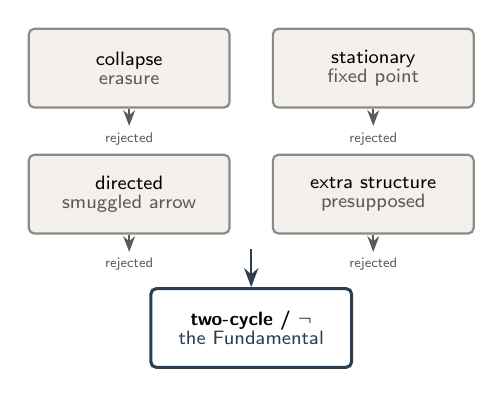
\begin{tikzpicture}[
  font=\scriptsize\sffamily,
  box/.style={
    draw=nodeedge, fill=nodefill, thick, rounded corners=2pt,
    minimum width=2.55cm, minimum height=1.0cm, align=center
  },
  kill/.style={box, draw=muted!70, fill=soft},
  live/.style={box, draw=accent, fill=white, line width=1.1pt},
  arr/.style={-{Stealth[length=2mm]}, muted, thick}
]
  \node[kill] (a) at (0,2.25) {collapse\\[-1pt]{\color{muted}erasure}};
  \node[kill] (b) at (3.1,2.25) {stationary\\[-1pt]{\color{muted}fixed point}};
  \node[kill] (c) at (0,0.65) {directed\\[-1pt]{\color{muted}smuggled arrow}};
  \node[kill] (d) at (3.1,0.65) {extra structure\\[-1pt]{\color{muted}presupposed}};
  \node[live] (e) at (1.55,-1.05)
    {\textbf{two-cycle / $\Neg$}\\[-1pt]{\color{accent}the Fundamental}};

  \foreach \n in {a,b,c,d} {
    \draw[arr] (\n.south) -- ++(0,-0.22);
    \node[muted] at ($(\n.south)+(0,-0.38)$) {\tiny rejected};
  }
  \draw[-{Stealth[length=2.4mm]}, accent, thick]
    (1.55,-0.05) -- (e.north);
\end{tikzpicture}%
}{Eliminative classification of self-actions.
Only the live, symmetric two-cycle---Boolean complement---survives.}

% ════════════════════════════════════════════════════════════
\section{The foundation is dynamic}
% ════════════════════════════════════════════════════════════

\begin{principle}{Principle 4}
The fundamental law has no fixed point.
\end{principle}

Reality is not a static being.
Reality is \term{perpetual distinction}.

\figblock{%
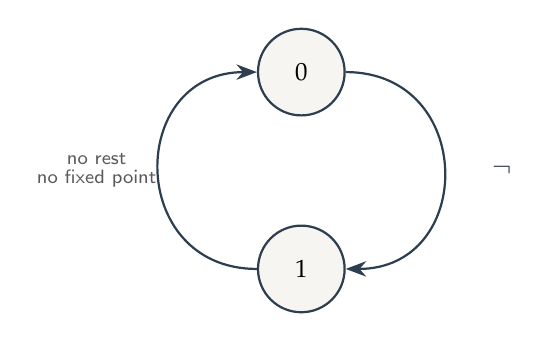
\begin{tikzpicture}[
  font=\small\sffamily,
  pole/.style={
    circle, draw=accent, fill=nodefill, thick,
    minimum size=1.1cm, inner sep=0pt
  }
]
  \node[pole] (T) at (0,1.25) {$0$};
  \node[pole] (F) at (0,-1.25) {$1$};
  \draw[-{Stealth[length=2.6mm]}, accent, thick]
    (T.east) to[out=0,in=0,looseness=1.7] (F.east);
  \draw[-{Stealth[length=2.6mm]}, accent, thick]
    (F.west) to[out=180,in=180,looseness=1.7] (T.west);
  \node[accent, font=\sffamily\bfseries] at (2.55,0) {$\Neg$};
  \node[muted, align=center, font=\scriptsize\sffamily] at (-2.6,0)
    {no rest\\[-1pt]no fixed point};
\end{tikzpicture}%
}{The law is a perpetual flip: every state is moved.
Nothing is left alone.}

% ════════════════════════════════════════════════════════════
\section{Self-reference leaves a blind spot}
% ════════════════════════════════════════════════════════════

\begin{principle}{Principle 5}
Self-reference inevitably generates a blind spot.
\end{principle}

Whenever a system attempts a complete description of itself,
there always remains a valid description external to that account.

This is the familiar pressure of self-reference and diagonalisation.

The universe is therefore \term{perpetually incomplete from within}.

\figblock{%
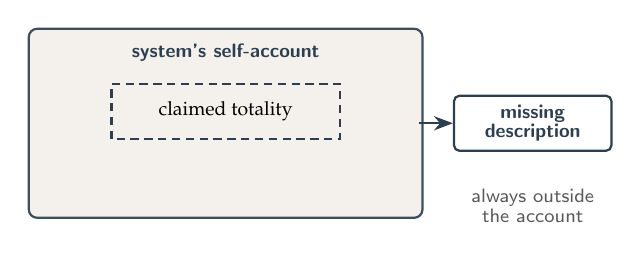
\begin{tikzpicture}[
  font=\small\sffamily,
  arena/.style={
    draw=nodeedge, thick, rounded corners=3pt, fill=soft,
    minimum width=5.0cm, minimum height=2.4cm
  }
]
  \node[arena] (A) at (0,0) {};
  \node[font=\sffamily\bfseries\scriptsize, text=accent] at (0,0.9)
    {system's self-account};
  \draw[accent, thick, densely dashed]
    (-1.45,-0.2) rectangle (1.45,0.5);
  \node[font=\scriptsize] at (0,0.15) {claimed totality};

  \node[draw=accent, fill=white, thick, rounded corners=2pt,
        minimum width=2.0cm, minimum height=0.7cm, align=center,
        font=\scriptsize\sffamily\bfseries, text=accent]
    (X) at (3.9,0) {missing\\[-1pt]description};
  \draw[-{Stealth[length=2.4mm]}, accent, thick]
    (2.45,0) -- (X.west);
  \node[muted, font=\scriptsize\sffamily, align=center] at (3.9,-1.05)
    {always outside\\[-1pt]the account};
\end{tikzpicture}%
}{Any total self-description leaves a residue.
Diagonalisation names that residue.}

% ════════════════════════════════════════════════════════════
\section{Growth is necessary}
% ════════════════════════════════════════════════════════════

\begin{principle}{Principle 6}
Growth is a necessary consequence of incompleteness.
\end{principle}

The only way to accommodate the missing description is to enlarge the arena.

% Linear chain + clear U-turn underneath (does not cross any node).
\figblock{%
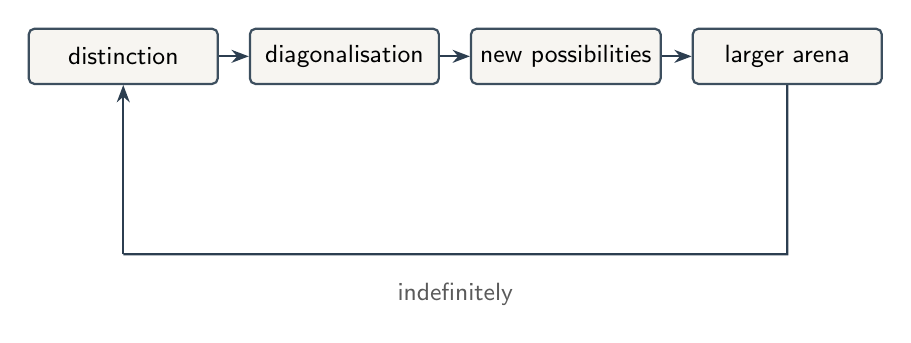
\begin{tikzpicture}[
  font=\small\sffamily,
  stepnode/.style={
    draw=nodeedge, fill=nodefill, thick, rounded corners=2pt,
    minimum height=0.7cm, minimum width=2.4cm, align=center
  },
  arr/.style={-{Stealth[length=2.2mm]}, accent, thick}
]
  \node[stepnode] (ndist)  {distinction};
  \node[stepnode, right=0.38cm of ndist] (ndiag) {diagonalisation};
  \node[stepnode, right=0.38cm of ndiag] (nnew)  {new possibilities};
  \node[stepnode, right=0.38cm of nnew]  (narena){larger arena};

  \draw[arr] (ndist) -- (ndiag);
  \draw[arr] (ndiag) -- (nnew);
  \draw[arr] (nnew)  -- (narena);

  % Deep U-turn. Vertical return aims at the geometric midpoint of the
  % bottom edge (not a corner). Label sits cleanly below the bar.
  \coordinate (distBot) at ($(ndist.south west)!0.5!(ndist.south east)$);
  \coordinate (underDist) at ([yshift=-2.15cm]distBot);
  \coordinate (underArena) at ([yshift=-2.15cm]narena.south);
  \draw[accent, thick] (narena.south) -- (underArena) -- (underDist);
  \draw[arr] (underDist) -- (distBot);
  \node[font=\small\sffamily, text=muted, anchor=north, yshift=-7pt]
    at ($(underArena)!0.5!(underDist)$) {indefinitely};
\end{tikzpicture}%
}{Growth is not an add-on. It is forced by incompleteness.}

% ════════════════════════════════════════════════════════════
\Needspace{12em}
\section{Records and archives}
% ════════════════════════════════════════════════════════════

\begin{principle}{Principle 7}
Records appear when distinctions are preserved.
\end{principle}

If evolution never destroys distinctions, then apparent forgetting must be
accompanied by hidden bookkeeping.

\begin{claimbox}
\centering
Loss implies archives.
\end{claimbox}

\Needspace{9em}
\figblock{%
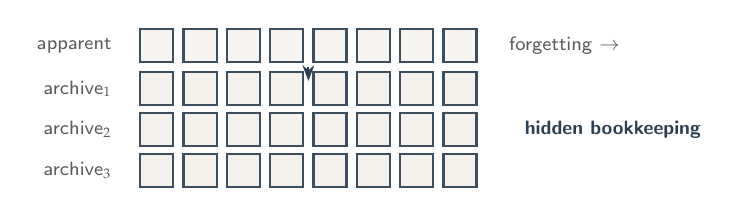
\begin{tikzpicture}[
  font=\scriptsize\sffamily,
  cell/.style={
    draw=nodeedge, fill=nodefill, thick, minimum size=0.42cm
  }
]
  \foreach \i in {0,...,7} {
    \node[cell] at (\i*0.55, 0.55) {};
  }
  \node[muted, left] at (-0.45,0.55) {apparent};
  \node[muted, right] at (4.35,0.55) {forgetting $\rightarrow$};

  \foreach \y/\lab in {0.0/{archive$_1$}, -0.52/{archive$_2$}, -1.04/{archive$_3$}} {
    \foreach \i in {0,...,7} {
      \node[cell, fill=soft] at (\i*0.55, \y) {};
    }
    \node[muted, left] at (-0.45,\y) {\lab};
  }
  \draw[-{Stealth[length=2mm]}, accent, thick]
    (1.925,0.28) -- (1.925,0.1);
  \node[accent, font=\sffamily\bfseries\scriptsize, anchor=west]
    at (4.55,-0.52) {hidden bookkeeping};
\end{tikzpicture}%
}{What seems lost is relocated.
Preservation of distinction forces an archive beneath the stream.}

% ════════════════════════════════════════════════════════════
\Needspace{14em}
\section{Time as reading}
% ════════════════════════════════════════════════════════════

\begin{principle}{Principle 8}
Time is the process of reading the archive.
\end{principle}

The archive itself has no intrinsic direction.
Observers define direction from their position within it.

The arrow of time is therefore not a fundamental property.
It is an \term{orientation on accumulated records}.

\figblock{%
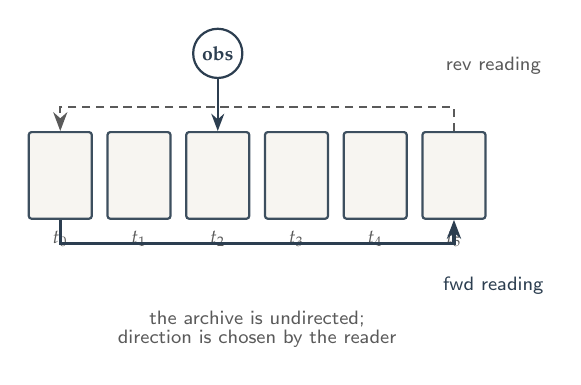
\begin{tikzpicture}[
  font=\small\sffamily,
  page/.style={
    draw=nodeedge, fill=nodefill, thick, rounded corners=1pt,
    minimum width=0.8cm, minimum height=1.1cm
  }
]
  \foreach \i in {0,...,5} {
    \node[page] (p\i) at (\i*1.0,0) {};
    \node[muted, font=\scriptsize] at (\i*1.0,-0.8) {$t_{\i}$};
  }
  \node[circle, draw=accent, fill=white, thick, inner sep=2pt,
        font=\scriptsize\bfseries, text=accent] (obs) at (2.0,1.55) {obs};
  \draw[-{Stealth[length=2.2mm]}, accent, thick] (obs) -- (p2.north);

  \draw[-{Stealth[length=2.4mm]}, accent, line width=1.1pt]
    (p0.south) -- ++(0,-0.3) -| (p5.south);
  \draw[-{Stealth[length=2.4mm]}, muted, densely dashed, thick]
    (p5.north) -- ++(0,0.3) -| (p0.north);

  \node[accent, font=\scriptsize\sffamily] at (5.5,-1.4) {fwd reading};
  \node[muted, font=\scriptsize\sffamily] at (5.5,1.4) {rev reading};

  \node[muted, font=\scriptsize\sffamily, align=center] at (2.5,-1.95)
    {the archive is undirected;\\[-1pt]
     direction is chosen by the reader};
\end{tikzpicture}%
}{The arrow of time is an orientation imposed by an observer,
not a property of the archive itself.}

% ════════════════════════════════════════════════════════════
\Needspace{10em}
\section{The subject is not an object}
% ════════════════════════════════════════════════════════════

\begin{principle}{Principle 9}
The most fundamental identity is not among the distinguished states.
\end{principle}

It is the act of distinction itself.

\begin{claimbox}
\centering
The true subject is identical with the lawful cut ---\\[0.15em]
not with any object it distinguishes.
\end{claimbox}

% ════════════════════════════════════════════════════════════
\Needspace{16em}
\section{Physics is downstream}
% ════════════════════════════════════════════════════════════

\begin{principle}{Principle 10}
Physics functions as a downstream interpretive dictionary.
\end{principle}

Matter, entropy, memory, measurement, observers, and spacetime are
interpretations of the bookkeeping generated by the preceding principles.
None of these elements constitute the foundation.

\figblock{%
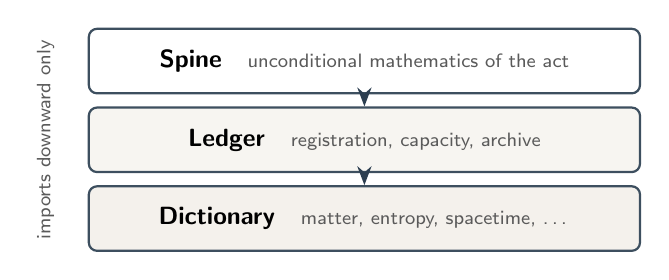
\begin{tikzpicture}[
  font=\small\sffamily,
  layer/.style={
    draw=nodeedge, thick, rounded corners=3pt,
    minimum width=7.0cm, minimum height=0.82cm, align=center
  }
]
  \node[layer, fill=white] (s) at (0,1.7)
    {\textbf{Spine}\quad{\color{muted}\scriptsize unconditional mathematics of the act}};
  \node[layer, fill=nodefill] (l) at (0,0.7)
    {\textbf{Ledger}\quad{\color{muted}\scriptsize registration, capacity, archive}};
  \node[layer, fill=soft] (d) at (0,-0.3)
    {\textbf{Dictionary}\quad{\color{muted}\scriptsize matter, entropy, spacetime, \ldots}};

  \draw[-{Stealth[length=2.4mm]}, accent, thick] (s) -- (l);
  \draw[-{Stealth[length=2.4mm]}, accent, thick] (l) -- (d);

  \node[muted, font=\scriptsize\sffamily, rotate=90] at (-4.05,0.7)
    {imports downward only};
\end{tikzpicture}%
}{Three layers, strict downward dependency.
Physical vocabulary lives at the bottom, as interpretation.}

% ════════════════════════════════════════════════════════════
\section*{Conclusion}
% ════════════════════════════════════════════════════════════

\hrthin

\begin{center}
\begin{minipage}{0.88\textwidth}
\large\itshape\color{accent}
The universe is not composed of discrete things.\\[0.3em]
It consists of distinctions perpetually engaged\\
in the process of self-differentiation.
\end{minipage}
\end{center}

\hrthin

% Keep the chain + glossary + end together on the final page.
\clearpage
\section*{How the steps hang together}

\figblock{%
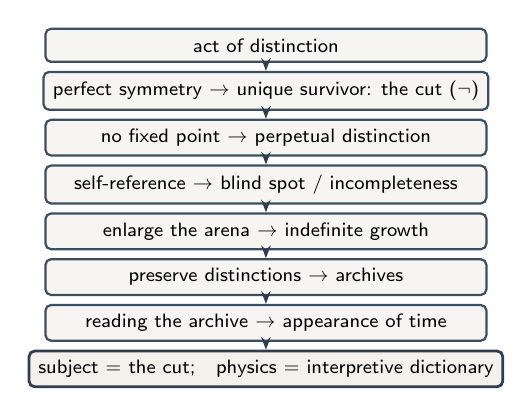
\begin{tikzpicture}[
  font=\scriptsize\sffamily,
  N/.style={
    draw=nodeedge, fill=nodefill, thick, rounded corners=2pt,
    minimum width=5.6cm, minimum height=0.42cm, align=center
  },
  arr/.style={-{Stealth[length=1.6mm]}, accent, thick}
]
  \node[N] (1) {act of distinction};
  \node[N, below=0.1cm of 1] (2) {perfect symmetry $\rightarrow$ unique survivor: the cut ($\Neg$)};
  \node[N, below=0.1cm of 2] (3) {no fixed point $\rightarrow$ perpetual distinction};
  \node[N, below=0.1cm of 3] (4) {self-reference $\rightarrow$ blind spot / incompleteness};
  \node[N, below=0.1cm of 4] (5) {enlarge the arena $\rightarrow$ indefinite growth};
  \node[N, below=0.1cm of 5] (6) {preserve distinctions $\rightarrow$ archives};
  \node[N, below=0.1cm of 6] (7) {reading the archive $\rightarrow$ appearance of time};
  \node[N, below=0.1cm of 7, fill=soft, draw=accent, line width=1pt] (8)
    {subject $=$ the cut;\quad physics $=$ interpretive dictionary};

  \foreach \a/\b in {1/2,2/3,3/4,4/5,5/6,6/7,7/8}
    \draw[arr] (\a) -- (\b);
\end{tikzpicture}%
}{The argument as a single descending chain.}

\vspace{0.45em}
\section*{An experimental annex}

Alongside the main development, the repository carries a small
quarantined annex of machine-checked probes; nothing in the main story
depends on them. They ask how far the two-letter alphabet carries on
its own. Every finite rhythm turns out to be exactly two flips of the
fundamental beat, and for plain rotations the two flips can be written
down in closed form. The circle of fifths closes after exactly twelve
steps --- proved as a fact about order, not sound --- and the general
law behind it (period equals size over greatest common divisor) is a
theorem. A wave equation lives natively on the alphabet: its step is
two bounces by definition, running it backwards is swapping the
bounces, and its spectrum is set by its boundary. Any state, under any
coupling, must return to itself within the capacity of its carrier ---
a small eternal return, forced by losslessness alone. And at the edge
of the ladder sits the space of complete histories, which no list can
exhaust, in which every rung embeds, and where --- unlike inside the
arena --- forgetting becomes possible. The annex records what it
cannot do as carefully as what it can: no continuum, no real
frequencies, and the closed-form wave-period law is left, honestly, as
a wall.

\vspace{0.45em}
\section*{Glossary}

\renewcommand{\arraystretch}{1.18}
{\footnotesize
\begin{tabularx}{\textwidth}{@{}>{\bfseries\sffamily\color{accent}}l X@{}}
\toprule
Term & Meaning here \\
\midrule
Distinction / cut
  & The minimal act that separates without preferring a side \\
Boolean complement ($\Neg$)
  & The unique minimal symmetric self-action that survives classification \\
Fixed point
  & A state the act leaves unchanged --- ruled out for the fundamental law \\
Diagonalisation
  & Self-reference forcing a description that cannot fit inside the current account \\
Arena / ladder
  & The growing space of possibilities opened by incompleteness \\
Archive / record
  & Preserved distinctions; the bookkeeping behind apparent loss \\
Arrow of time
  & An orientation chosen by an observer reading the archive --- not a primitive \\
Subject
  & The act of distinction itself, not any distinguished object \\
Dictionary
  & Downstream physical readings (matter, entropy, spacetime, \ldots)
    of the bookkeeping \\
\bottomrule
\end{tabularx}
}

\vspace{0.55em}
\begin{center}
  {\color{rule}\rule{0.25\textwidth}{0.4pt}}\\[0.3em]
  {\color{muted}\scriptsize End.}
\end{center}

\end{document}
